The optimizations performed by \Treebeard{} at the low-level IR are presented in this section.

\subsection{Vectorization}
\label{sec:Vectorization}
\Treebeard{} specializes the tree walk over a tiled tree to make use of vector instructions. 
%Vectorization performed by Treebeard is enabled by the tiling transformations described in section \ref{sec:Tiling}. 
This specialization happens as we lower low level IR to LLVM IR.  These are then converted to vector instructions in the target ISA by 
the LLVM JIT.

The below listing shows the low-level IR for a vectorized tree walk in detail. 
\begin{lstlisting}[style=c++]
  // A lookup table that determines the child index of
  // the next tile given the tile shape and the outcome
  // of the vector comparison on the current tile
  int16_t LUT[NUM_TILE_SHAPES, pow(2, TileSize)]
  
  WalkDecisionTree(...) {
    tile = getRoot(tree)
    while (isLeaf(tree, tile)==false) do {
      thresholds = loadThresholds(tree, tile)
      featureIndices = loadFeatureIndices(tree, tile)
      // Gather required feature from the current row
      features = rows[i][featureIndices]
      // Vector comparison of features and thresholds
      comparison = features < thresholds
      
      // Pack bits in comparison vector into an integer
      comparisonIndex = combineBitsIntoInt(comparison)
      
      // Get child index of tile we need to move to
      tileShape = loadTileShape(tree, tile)
      childIndex = LUT[tileShapeID, comparisonIndex]
      
      // Move to the correct child of the current node
      tile = getChildTile(tree, tile, childIndex) 
    }
    prediction = getLeafValue(tile)
  }  
\end{lstlisting}

When lowering to LLVM, operators \op{loadThresholds} and \op{loadFeatureIndices} (lines 11 and 13) are lowered to use vectorized load instructions. Predicates are then evaluated using vector comparison instructions (lines 15 to 18). 
The next step is to determine which child to visit (lines 21 to 25), as we explain below this depends not only on the result of the comparison but also on the shape of the sub-tree that the tile represents.

\CommentOut{
To evaluate the current tile, the vector of thresholds is first loaded (\texttt{loadThresholds}).
Then, the features required for comparison are gathered into a vector. The feature 
vector is compared to the threshold vector and the child tile to move to is determined (lines 15 to 25).
More details about tile shapes and the look up table are presented in subsequent sections.
}

\begin{figure}
  \centering
  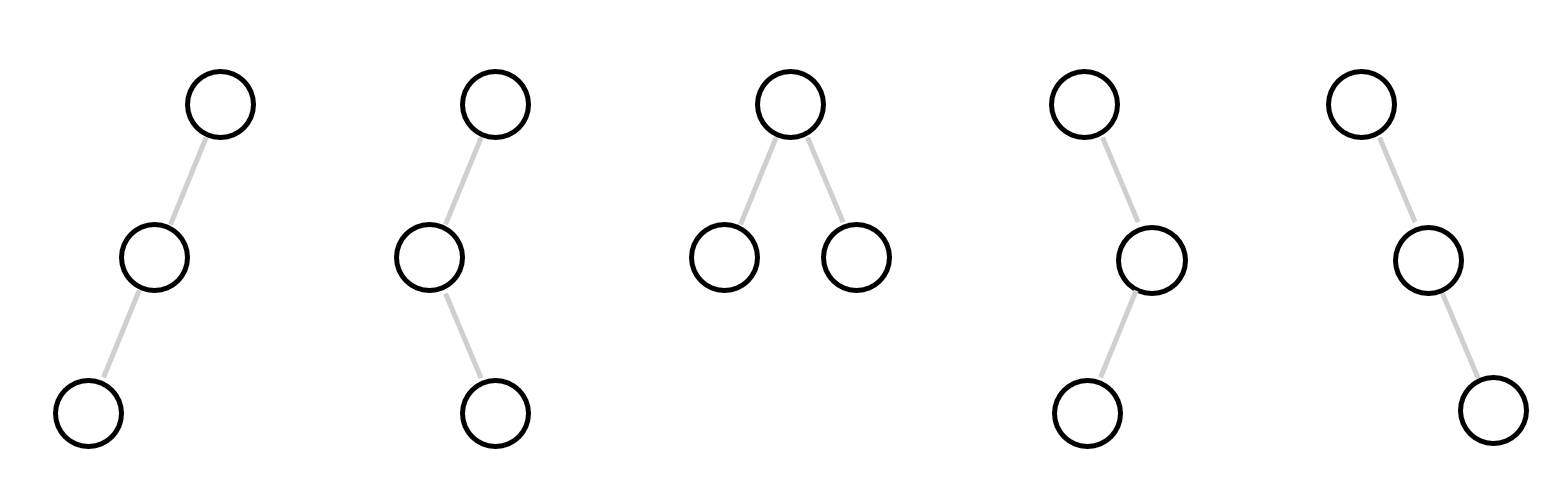
\includegraphics[width=\linewidth]{figures/TileShapes_Size3.PNG}
  \caption{All possible tile shapes with tile size $n_t=3$.}
  \label{Fig:TileSize3Shapes}
\end{figure}

\subsubsection{Tile Shapes and Tree Traversal}
\label{Sec:TileShapesAndDecisionTreeInference}
%We refer to the shape of the region that encloses all nodes in a tile in a diagram of the decision tree as the \textbf{\emph{tile shape}}.
For a given tile size $n_t$, each unique legal binary tree containing $n_t$ nodes (nodes being indistinguishable) corresponds to
a \textbf{\emph{tile shape}}. Figure \ref{Fig:TileSize3Shapes} enumerates all tile shapes with a tile size of 3. 
\CommentOut{
% There are a total of 5 tile shapes with size 3. The number of tile shapes with a tile size $n_t$, denoted by $NTS(n_t)$ is given by the following equation. 

% \begin{equation}
%   NTS(n) = \sum_{k=0}^{n-1} NTS(k) \times NTS(n-k-1)
% \end{equation}

% where $NTS(0) = NTS(1) = 1$.

\subsubsection{Tile Shapes and Decision Tree Inference}
\label{Sec:TileShapesAndDecisionTreeInference}
\Treebeard{} uses vector instructions to accelerate decision tree walks. Vector instructions are used to evaluate the predicates
of all the nodes in a tile simultaneously. However, once the predicates of all the nodes in the tile are evaluated, computing
the next tile to move to, given the outcome of the comparison depends on the tile shape of the current tile. To illustrate 
this problem, consider the case of the tiles of size 3 shown in Figure \ref{Fig:TileTraversalTileSize3}.
}

%% To understand how tile shapes influence the outcome of tile evaluation, consider the case of the tiles of size 3 shown in figure \ref{Fig:TileTraversalTileSize3}
\begin{figure}
  \centering
  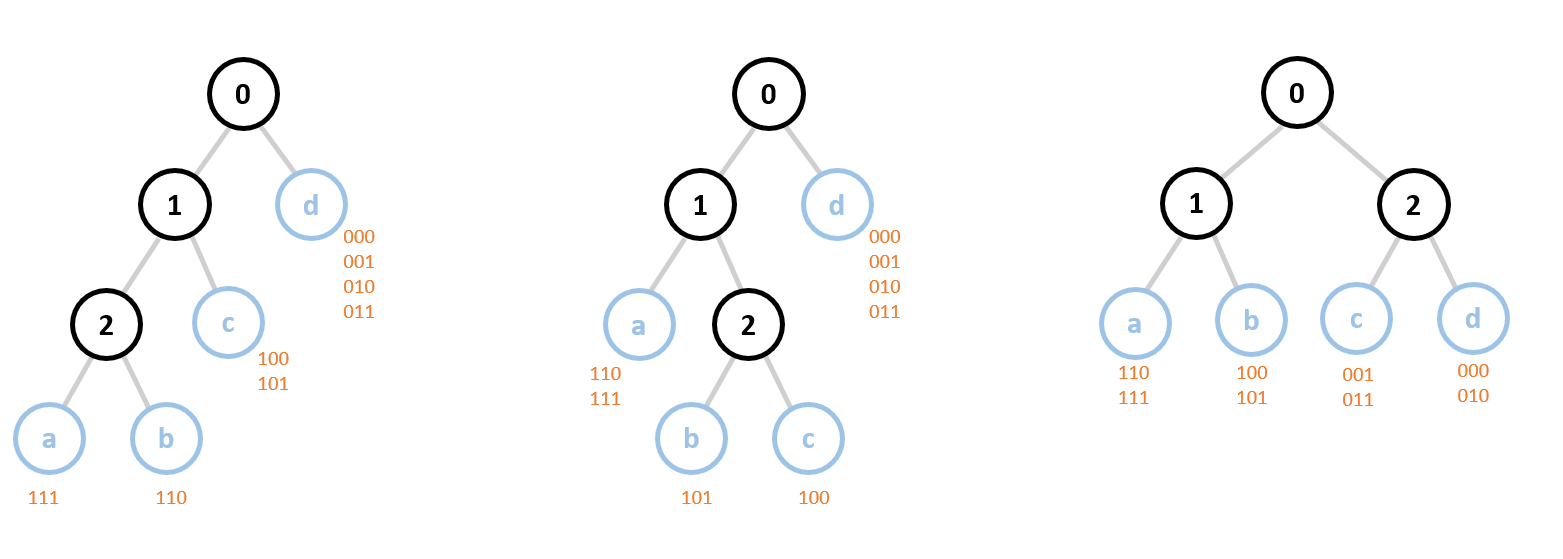
\includegraphics[width=\linewidth]{figures/TileTraversal_Size3.PNG}
  \caption{Example tile traversals with tile size $n_t=3$.}
  \label{Fig:TileTraversalTileSize3}
\end{figure}
%% The diagram 
Given the  comparison vector evaluated for a tile, the tile that needs to be traversed next depends
on the shape of the tile. To understand this, consider Figure~\ref{Fig:TileTraversalTileSize3} that 
shows 3 of the 5 possible tile shapes for a tile size of 3. The nodes drawn in black are members of the tile.
The nodes in blue are the root nodes of the children tiles.
% To traverse a tile on an input row, first, the predicate of each node in the tile is computed. Subsequently, we need to determine which of the child tiles to move to next. Note that a true predicte (bit value 1) on a node implies a move to the left child and a false predicate (bit value 0) implies a move to the right child.
The bit strings (written in red) show which child 
%% we need to move to
needs to be traversed next,  given the outcomes of the comparison.
The bits represent the comparison outcomes of nodes -- the MSB is the predicate outcome of node 0 and the LSB the predicate
outcome of node 2. For example, for the first tile shape, if the comparison outcome is 111, the next node to evaluate is $a$. 
% However, if the predicate of node 1 is false, then we need to move to $d$ regardless of the outcomes of nodes 2 and 3.
It is easy to see that, depending on the tile shape, the same comparison outcomes can mean moving to different children.
For example, for the outcome 011, the next tile is the 4th child (node $d$) for the first two tile shapes while it is 
the 3rd child for the other tile shape (node $c$)\footnote{Children of a tile are ordered left to right regardless of depth.}.

\subsubsection{Lookup Table}
\label{sec:LookupTable}
As illustrated above a combination of tile shape and the comparison outcome can be used to determine the child to visit. 
We introduce an additional map called a lookup table (LUT) to encode this information:
\[
LUT : (TileShape, \{0, 1\}^{n_t}) \rightarrow [0, n_t] \subset \mathbb{N}.
\]
The LUT is indexed by 
the tile shape and the comparison outcome. 
where $n_t$ is the tile size, $\{0, 1\}^{n_t}$ is a vector of $n_t$ booleans. The value returned by the LUT is the index of
the child of the current tile that should be evaluated next. For example, if we are evaluating the first tile $T_1$ in 
Figure \ref{Fig:TileTraversalTileSize3}, and the result of the comparison is 110, then $LUT(TileShape(T_1), 110)=2$ since 
the tile %% we need to evaluate 
to be traversed next is the tile with node $b$, which is the second child of the current tile.

In order to realize this LUT in generated code, \Treebeard{} associates a non-negative integer ID with every unique tile shape of the
given tile size. The result of the comparison, a vector of booleans, can be interpreted as a 64-bit integer. Therefore, the LUT
can be implemented as a 2 dimensional array. \Treebeard{} computes the values in the LUT statically as the tile size is a compile time constant.
% \begin{lstlisting}{style=c++}
%   int16_t LUT[NTS(n_t), pow(2, n_t)]  
% \end{lstlisting}

\subsection{In-Memory Representation of Tiled Trees}
\label{Sec:MemoryRep}
\Treebeard{} currently has two in-memory representations for tiled trees - an array based representation and a sparse representation.
Both representations use an array of \texttt{structs} to represent the model. 

\subsubsection{Array-Based Representation}
\label{sec:ArrayBased}
Each tree in the model is represented as an array of tiles using the standard representation of trees as arrays. The root node is 
at index 0 and for a node at index $n$, the index of its $i^{th}$ child\footnote{Nodes
in the tree of tiles have $n_t + 1$ children.} is given by $(n_t + 1) n + (i + 1)$.
% A tile is represented by an object of the following struct.
% \begin{lstlisting}{style=c++}
%   struct Tile {
%     // A vector of TileSize elements
%     <ThresholdType x TileSize> thresholds; 
%     <FeatureIndexType x TileSize> featureIndices;
%     // Integer that identifies the tile shape
%     TileShapeIDType tileShapeID; 
%   };  
% \end{lstlisting}
% \TODO{AP Is this level of detail really needed? Also, the vector type notation needs to be introduced somewhere.}
Even though this representation is simple and efficient for small models, the memory required for bigger models is very large. 
%The memory footprint is up to 20X that of the scalar representation.
This memory bloat causes performance problems due to L1 cache and L1 TLB misses.
%because the span of the L1 TLB is not sufficient to efficiently translate addresses for the whole model.
Storing leaves as full tiles (even though they represent a single value) and the
empty space introduced due to the array based representation of trees that 
are not complete account for most of the increase.
%The sparse representation described next tries to address these issues. 

\subsubsection{Sparse Representation}
\label{sec:SparseRep}
We reduce the large memory footprint of the array based representation by doing the following.

\begin{itemize}
  \item We add a child pointer to each tile to eliminate the wasted space in the array representation. This 
  points to the first child of the tile. All children of a tile are stored contiguously.
  \item Leaves are stored as a separate array of scalar values. Across all our benchmarks, after tiling a large fraction of 
  leaves are such that all their siblings are also leaves. Such leaves are directly moved into the leaves array. For leaves
  for which this property does not hold, an extra ``hop'' is added by making the original leaf tile a normal tile. All its
  children are leaves with the same value as the original leaf.
\end{itemize}

\begin{figure}
  \centering
  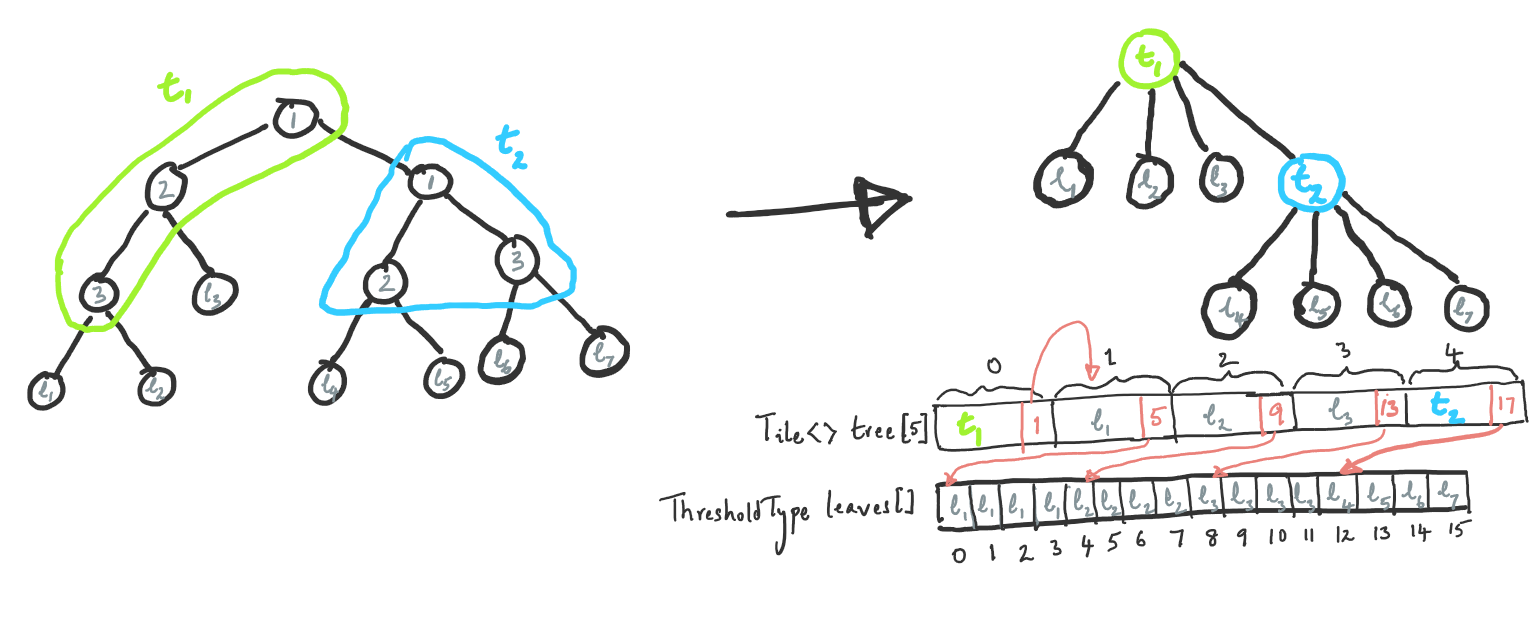
\includegraphics[width=\linewidth]{figures/SparseRep_TileSize3.PNG}
  \caption{Sparse representation with tile size $n_t=3$. Leaves $l_4$, $l_5$, $l_6$ and $l_7$ are moved into the \op{leaves} array.
  Extra hops are added for $l_1$, $l_2$ and $l_3$ as $t_2$ is a non-leaf tile. The new leaves added as children of $l_1$, $l_2$ and $l_3$
  are moved to the \op{leaves} array.}
  \label{Fig:SparseRep}
\end{figure}

Figure \ref{Fig:SparseRep} shows the details of the sparse representation.
% The tree on the left of the diagram is the actual decision tree with the nodes grouped into tiles $t_1$ and $t_2$. The tree on the right is the tree of tiles.
The arrays depicted below show how the tree is represented in memory. The first array ($\texttt{tree}$) is an array of tiles 
and has 5 elements. Each element of the array represents a single tile and has the thresholds of the nodes, the feature
indices, a tile shape ID and a child pointer (shown as red arrows). The second array, \op{leaves}, contains
all leaf values. 

%%%% COMMENT START %%%%% 

\CommentOut{
As a specific example, consider the tile $t_1$. The tile has four children -- $l_1$, $l_2$, $l_3$ and $t_2$ in that order (left to right). These tiles are stored contiguously in the $\texttt{tree}$ array and a pointer to the first of these, $l_1$ is stored in the tile $t_1$ (the index 1 is stored in the tile $t_1$ as shown). 

Now consider the tile $t_2$. Since all children of the tile $t_2$ are leaves, they are all moved into the $\texttt{leaves}$ array.
To store a pointer into the $\texttt{leaves}$ array, we add $\texttt{len(tree)}$ to the element index in the $\texttt{leaves}$ array.
The tile $t_2$'s child is the element at index 12 of the $\texttt{leaves}$ array. Therefore, the index $12 + 5 = 17$ is stored in 
the tile $t_2$. Any index $i$ that is greater than the length of the $\texttt{tree}$ array is regarded as an index into the
$\texttt{leaves}$ array. The index into the $\texttt{leaves}$ array is $i - \texttt{len(tree)}$.

The other aspect of the representation is that an extra hop is added for the leaves $l_1$, $l_2$ and $l_3$ in order to simplify
code generation. This enforces the invariant that all leaves are stored in the leaves array and  simplifies checking whether
we've reached a leaf. Therefore, 4 new leaves are added as children for each of the original leaves $l_1$, $l_2$ and $l_3$. 
Each of these 12 newly added leaves has the same value as its parent. These are the first 12 elements of the $\texttt{leaves}$ array.

Even though we currently have implementations of the two representations detailed in sections \ref{sec:ArrayBased} 
and \ref{sec:SparseRep}, support for other representations is not hard to add. All optimizing passes that work on 
the high level and mid level IR will continue to work as is. Programmers need only provide new lowering passes for
a few operations in the low level IR.

\subsubsection{Code Generation for Probability-Based Tiling}
As probability-based tiling pulls the most probable leaves of a decision tree nearest the root, it poses 
some implementation challenges. By design, the tiling process makes the tree of tiles 
imbalanced. The array based representation (section \ref{sec:ArrayBased})
cannot be used because of the memory footprint increase (a large part of the tree is empty, but would need to be allocated).
On the other hand, the sparse representation in section \ref{sec:SparseRep} adds 
an extra hop for leaves that have non-leaf siblings. But this would mean that we add extra hops for 
the most probable leaves after probability-based tiling which defeats the optimization.
\TODO{kr: connect to Peeling in MIR}
We address these challenges using a code generation strategy. Treebeard peels 
the tree walk and specializes the leaf checks at higher levels to avoid the extra hop. Currently, 
we determine the maximum depth of leaves needed to cover 90 percent of the inputs and peel the tree 
walk by as many iterations. For example, consider the case where leaves until depth 2 are needed to 
cover 90 percent of the training input. Then, Treebeard generates the following IR. 

\begin{lstlisting}{style=c++}
    // ...
    tree = getTree(forest, t)
    node = getRoot(tree)
    node = traverseTreeTile(tree, node, rows[i])
    if (isLeafTile(node)) {
        treePrediction = getLeafValue(tree, node)
    } else {    
        node = traverseTreeTile(tree, node, rows[i])
        if (isLeafTile(node)) {
            treePrediction = getLeafValue(tree, node)
        } else {    
            // Loop based traversal 
        }
    }
    treePrediction = getLeafValue(tree, node)
    // ...
\end{lstlisting}

The if statements check whether a node is a leaf tile and hence avoid the extra hop. 
%The memory 
%requirement is also not increased because only a small fraction of leaves are represented as full tiles.
While walk peeling is used to improve the performance of probability-based tiling by specializing leaf tests,
the transformation is by itself general and can be used in different contexts. For example, it could be used 
to elide leaf checks until a depth $d$ is reached if we know all leaves are at a depth greater than $d$. 

One other issue that the code generator needs to handle is that walks of different trees in the same ensemble may 
need to be peeled to different depths. A strategy similar to what is used for basic tiling is used to handle this.
Trees are reordered so that all trees 
with equal peeling depth are grouped together and the loops in the IR are fissed so that tree walks 
for these groups of trees can be specialized differently.
% This is very similar to the code generation strategy used for basic tiling.
}

%%%% COMMENT END %%%%%
